\documentclass{article}
\usepackage{graphics}
\newcommand\LuaLaTeX{Lua\LaTeX}

\begin{document}
\section{Documentation}

When you load the package \texttt{lua-visual-debug} in your \LuaLaTeX\ document (or use \verb|\input lua-visual-debug.sty| in plain \TeX), Lua\TeX\ will highlight boxes, penalties, glues and kerns in the PDF. This package requires you to process the document with \LaTeX\ (plain and LaTeX formats).

\begin{verbatim}
\documentclass{article}
\usepackage{lua-visual-debug}

\listfiles
\setlength\textwidth{300pt}
\setlength\textheight{10cm}

\begin{document}

A wonderful serenity has taken possession of my entire soul, like these sweet 
mornings of spring which I enjoy with my whole heart. I am alone, and feel the 
charm of existence in this spot, which was created for the bliss of souls like 
mine. I am so happy, my dear friend, so absorbed in the exquisite sense of mere 
tranquil existence, that I neglect my talents.


\bgroup\fontsize{30}{34}\selectfont
\centerline{\TeX}
\egroup

\vbox{\strut Hello}\kern .5cm\vbox{\strut World}

\[ e=mc^2 \]

\includegraphics[width=4cm]{cow}
\end{document}
\end{verbatim}

yields \vspace{5mm}

\noindent 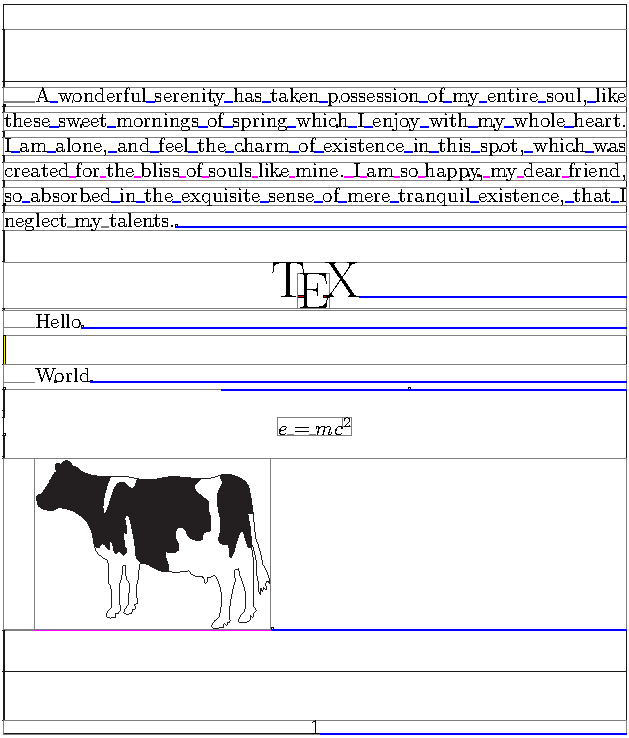
\includegraphics{lvdebug-sample.pdf}

\section{Copying}

Copyright 2012 Patrick Gundlach (patrick@gundla.ch), licensed under the MIT license. See the Lua file for details.


\end{document}
